\scanpage{211}
\mspage{210}
\uline{Questions}
\margin{À revoir}
\figure{\begin{tikzpicture}\draw[line width=.25pt] (0,0)..controls(.35,4)and(.4,7)..(.25,10);\end{tikzpicture}}

\figure{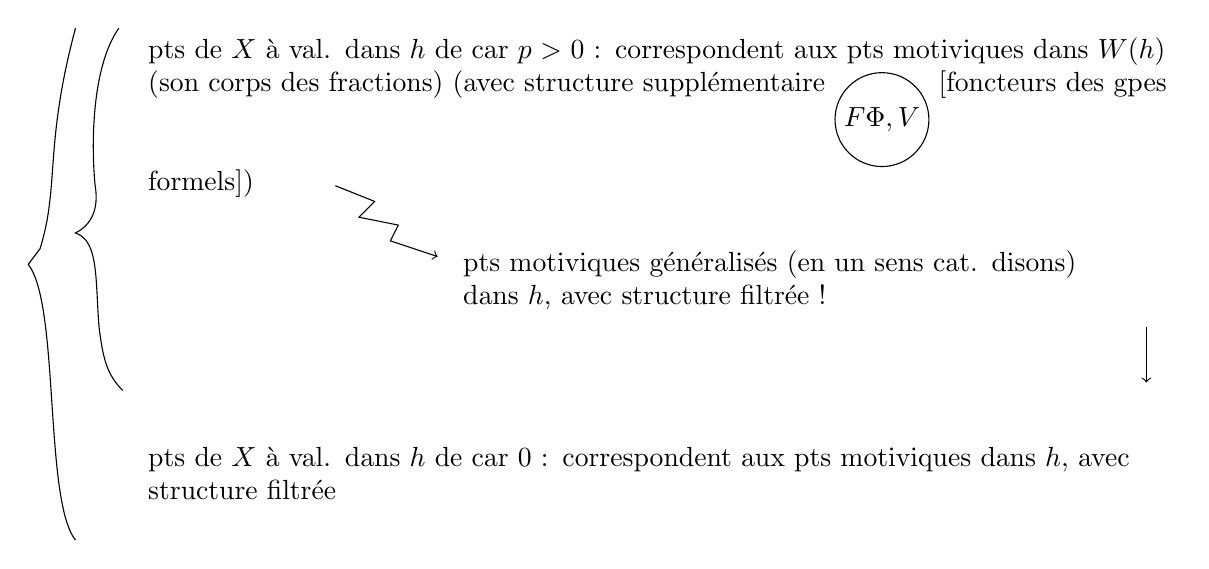
\begin{tikzpicture}[x=1cm,y=1cm]
\node[anchor=north west,text width=13cm] (p) at (0,0) {pts \inserted{de $X$} à val. dans $h$ \inserted{de car $p>0$} : correspondent aux pts motiviques \inserted{dans $W(h)$ (son corps des fractions)} (avec \uline{structure supplémentaire} \tikz[baseline=-.5ex]{\node[draw,circle,inner sep=2pt] {$F\deleted{\unsure{\Phi}},V$};} [\unsure{foncteurs} des gpes formels])};
\node[anchor=north west,text width=8cm] (q) at (4,-2.7) {pts motiviques généralisés (\unsure{en un sens} cat. disons) dans $h$, avec structure filtrée !};
\node[anchor=north west,text width=13cm] (r) at (0,-5.2) {pts \inserted{de $X$} à val. dans $h$ de car $0$ : correspondent aux pts motiviques dans $h$, avec \uline{structure filtrée}};
\draw[->] (2.5,-2) -- (3,-2.2) -- (2.8,-2.4) -- (3.3,-2.5) -- (3.2,-2.7) -- (3.8,-2.9);
\draw (-.25,0) .. controls (-.6,-.5) and (-.6,-1.5) .. (-.55,-2) .. controls (-.5,-2.3) and (-.6,-2.5) .. (-.8,-2.6) .. controls (-.5,-2.7) and (-.55,-3.2) .. (-.5,-3.8) .. controls (-.45,-4.2) and (-.4,-4.4) .. (-.2,-4.6);
\draw (-.8,0) .. controls (-1.2,-1.5) and (-1,-2) .. (-1.25,-2.8) -- (-1.4,-3) .. controls (-1,-3.5) and (-1.2,-6) .. (-.8,-6.5);
\draw[->] (12.8,-3.8) -- (12.8,-4.5);
\end{tikzpicture}}

\figure{\begin{tikzpicture}
\node[anchor=north west,text width=14cm] at (0,0) {pts \inserted{de $X$} à valeurs dans $C$ mod conj. complexe (= place) $\longleftrightarrow$ pts \inserted{motiviques} à valeurs dans \tikz[baseline=-.5ex]{\node[draw,circle] {$\mathbb R$};}, ou\\
à valeurs dans \tikz[baseline=-.5ex]{\node[draw,ellipse] {$\mathbb C$ avec \tikz[baseline=-.5ex]{\node[draw,circle] {$f_\infty$};}};}, ou\\
à valeurs dans $\mathbb Z$};
\draw (-.2,0) -- (-.2,-3);
\end{tikzpicture}}

\uline{\deleted{\unsure{de X}} \unsure{car $p$}}

\uline{Pts banaux}\qquad Pts à valeurs dans
\figure{
\begin{tikzpicture}\node[draw,circle] {$\mathbb Z_\ell$};\end{tikzpicture}},
$\ell$ premier avec car résiduelles.

ou \figure{
\begin{tikzpicture}\node[draw,circle] {$\mathbb Q_\ell$};\end{tikzpicture}}

\figure{\begin{tikzpicture}\draw[->] (0,1) -- (0,0);\end{tikzpicture}}
\uline{Cas particulier important}\quad \uline{Pts à valeurs dans corps}
fini $\mathbb F_q$ correspondent aux pts à valeurs dans le
\figure{\begin{tikzpicture}\node[draw,ellipse] {$W(\mathbb F_q)$};\end{tikzpicture}},
avec structure supplémentaire $(F,V)$
